\documentclass[10pt,landscape]{article}
\usepackage{amssymb,amsmath,amsthm,amsfonts}
\usepackage{multicol,multirow}
\usepackage{calc}
\usepackage{graphicx}
\usepackage{ifthen}
\usepackage[landscape]{geometry}
\usepackage[colorlinks=true,citecolor=blue,linkcolor=blue]{hyperref}


\ifthenelse{\lengthtest { \paperwidth = 11in}}
    { \geometry{top=.5in,left=.5in,right=.5in,bottom=.5in} }
	{\ifthenelse{ \lengthtest{ \paperwidth = 297mm}}
		{\geometry{top=1cm,left=1cm,right=1cm,bottom=1cm} }
		{\geometry{top=1cm,left=1cm,right=1cm,bottom=1cm} }
	}
\pagestyle{empty}
\makeatletter
\renewcommand{\section}{\@startsection{section}{1}{0mm}%
                                {-1ex plus -.5ex minus -.2ex}%
                                {0.5ex plus .2ex}%x
                                {\normalfont\large\bfseries}}
\renewcommand{\subsection}{\@startsection{subsection}{2}{0mm}%
                                {-1explus -.5ex minus -.2ex}%
                                {0.5ex plus .2ex}%
                                {\normalfont\normalsize\bfseries}}
\renewcommand{\subsubsection}{\@startsection{subsubsection}{3}{0mm}%
                                {-1ex plus -.5ex minus -.2ex}%
                                {1ex plus .2ex}%
                                {\normalfont\small\bfseries}}
\makeatother
\setcounter{secnumdepth}{0}
\setlength{\parindent}{0pt}
\setlength{\parskip}{0pt plus 0.5ex}
% -----------------------------------------------------------------------

\title{COMPSCI 2ME3 Cheat Sheet - young2}

\begin{document}

\raggedright
\footnotesize

\begin{center}
     \Large{\textbf{Geon's 2ME3 Cheat Sheet}} \\
\end{center}
\begin{multicols}{3}
\setlength{\premulticols}{1pt}
\setlength{\postmulticols}{1pt}
\setlength{\multicolsep}{3pt}
\setlength{\columnsep}{2pt}

\section{Introduction}
\subsection{Paradigms}
OO: C\#, C++, Python, Java, Scala\\
functional/declarative: Haskell, Elm, Scala\\
procedural/imperative: C, Assembly\\
logical: Prolog
\subsection{Why Java}
$$\begin{array}{l|l}
\text{Pros} & \text{Cons}\\
\hline
\text{Documentation} & \text{Too verbose}\\
\text{Portability} & \text{Big, worse performance}\\
\text{Very OO} & \text{Very OO}\\
\text{Some luxuries} & \text{Less control}
\end{array}$$
\subsection{Soft Eng}
Iron ring: Attended Kipling ceremony.\\
PEO (Professional Engineers of Ontario (P. Eng)): Requires practical experience and ethics exams. Controls right of practice and right to title.\\
CEAB (Canadian Engineering Accreditation Board): Determines if an engineering program gets approved.
\section{Software Development Life Cycle}
\textbf{Requirements Analysis}: What the software does. Placed into a \textit{software requirement specification} document.\\
\qquad Functional requirements: things the software actually does (should be atomic, precise, and verifiable).\\
\qquad Nonfunctional requirements: hard to verify (usabiliy, performance, security, reliability).\\
\textbf{Specification and Design}: How the program meets the requirements from the SRS document (modules, classes, packages, libraries, and class diagrams).\\
\textbf{Implementation} (coding)\\
\textbf{Validation and verification} (testing)\\
\textbf{Deployment and maintenance}\\
\subsection{Waterfall}
Perform each step of SDLC perfectly before moving to the next step. Idealistic since you have to go back and forth in practice.
\subsection{Agile (scrum, sprint)}
Similar to waterfall, but work in \textit{sprints}.\\
\textbf{Sprint}: one cycle of the agile SDLC where you work on a subset of requirements and cycle between RA, SD, implementation, and VV.\\
\subsection{Spiral}
Similar to agile, but make a prototype with each sprint cycle and hope the last one meets all the requirements. Get feedback on the prototypes after each cycle. What we did in 1XD3. 
\subsection{Good software}
\textbf{Maintainable}: Scalable, extendable, reusable.\\
\textbf{Reliable}.\\
\textbf{Correct}: Meets the SRS.\\
\textbf{Robust}: Meets the unspecified requirements.\\
Maintainability is important since 40\% of cost is development and 60\% is maintenance (20\% corrective, 20\% adaptive, 60\% improvements).
\section{OO}
\subsection{Encapsulation (information hiding)}
Safeguard the internal contents of a class from direct outside access. Make certain fields private and access them through public getters and setters.
\subsection{Inheritance (is-a)}
If A is-a B then A is built off of (extends) B. Good for reusability since code doesn't have to be rewritten.
\subsubsection{Association}
Relationship between two unrelated classes. Only associated through their objects, where each can exist without the other. 
\subsubsection{Aggregation (has-a)}
If A has-a B then A has an instance of B as a global variable.
\subsubsection{Composition (part-of)}
If A part-of B then A can't exist without B and neither can B exist without A. 
\subsubsection{Dependence (uses-a)}
If A uses-a B then A creates an object of B inside a method.
\subsection{Abstraction}
Hide complexity from users and only show relevant information. Hide implementation details using abstract (partial) classes or interfaces (full).
\subsection{Polymorphism}
Performing a certain action in different ways.\\
\textbf{Method overloading}: various methods with the same name but different parameters.\\
\textbf{Method overriding}: child class overrides a method of its parent.\\
\section{Class Diagrams}
3 sections in each box for a class: name, variables, functions.\\
$+$ for public, $-$ for private, $\#$ for protected.\\
{\centering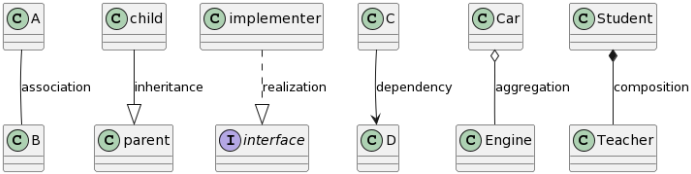
\includegraphics[scale=0.4]{img/UML.png}\par}
\section{Design Patterns}
\subsection{Decorator}
Dynamically add functionality and behaviour to objects without affecting the behaviour of other objects from the same class.\\
\quad Makes it easier to change or add a feature to existing objects for open-close principle and maintainability.\\
{\centering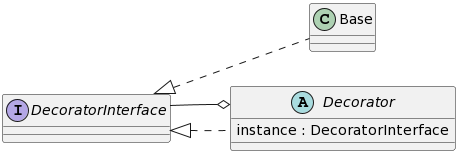
\includegraphics[scale=0.4]{img/decorator.png}\par}
\subsection{Factory}
Create objects while hiding the creation logic to the client and the client uses the same common interface to create a new type of object.\\
\quad Allow clients to create objects through a function instead of its actual constructor (i.e., not using \texttt{new})\\
{\centering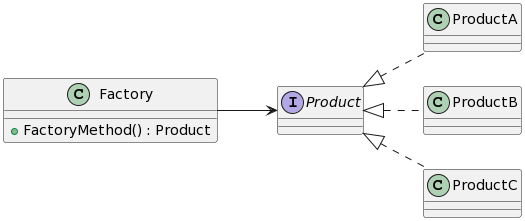
\includegraphics[scale=0.4]{img/factory.png}\par}
\subsection{Strategy}
Encapsulation of algorithms. Define a set of algorithms, each in their own class, and let their objects be interchangeable (i.e., they all inherit from a class or interface). Similar to factory but not hiding object creation and you need a function implemented by these classes. Allows algorithms to be swapped out at runtime.\\
{\centering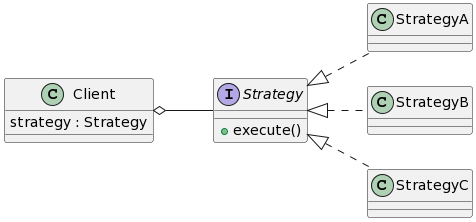
\includegraphics[scale=0.4]{img/strategy.png}\par}
\subsection{Observer}
Subjects maintain a list of observers and automatically notifies them of any state changes. Observers can unsub and resub to the subject. Variations of observers:\\
\textbf{Push}: subject updates observers.\\
{\centering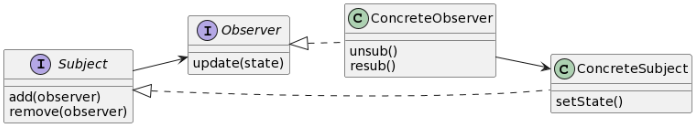
\includegraphics[scale=0.4]{img/observer_push.png}\par}
\textbf{Pull}: subject notifies observers a change was made, but the observer decides when to request that information.\\
{\centering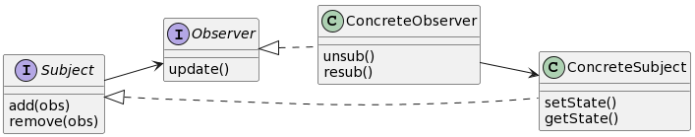
\includegraphics[scale=0.4]{img/observer_pull.png}\par}
\textbf{Poll}: the observer asks subject if things have changed.\\
\subsection{Singleton}
Allows you to limit a class to have only a single (or 0) instance through a private constructor. Allows for lazy instantiation where you don't actually instantiate it until you need it. Allows other classes to be extended with this pattern.\\
{\centering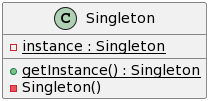
\includegraphics[scale=0.4]{img/singleton.png}\par}
\begin{verbatim}
public class Singleton {
    private static Singleton instance;
    
    public static Singleton getInstance() {
        if (instance == null) instance = new Singleton();
        return instance;
    }
    
    private Singleton() { // set up class }
}
\end{verbatim}
\subsection{Adapter}
A wrapper for a class that hides the implementation details (e.g. the data structure being used) of that class. Can be used to encapsulate data interface. E.g. service is \texttt{ArrayList} and the adapter implements \texttt{get} and \texttt{set} for \texttt{ArrayList}.\\
{\centering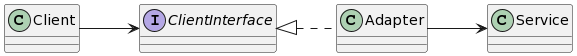
\includegraphics[scale=0.4]{img/adapter.png}\par}
\subsection{Proxy}
Similar to adapter, but the service also implements the interface and the client uses the proxy instead of the service directly for security and performance. E.g. preprocessing, denying execution, etc. before the proxy sends it to the service. You can have multiple proxies that implement different reasons to use the proxy (e.g. different ones for security and performance). You can control access to the original object, allowing you to interfere either before or after the request gets through to the original object without changing the service class.\\
{\centering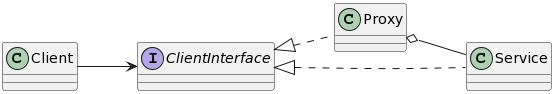
\includegraphics[scale=0.4]{img/proxy.png}\par}
\subsection{Command}
Encapsulate all information needed to perform an action or trigger an event at a later time. Information includes method name, the object that owns the method and values for the method parameters. Similar to adapter, but \texttt{Remote} requires an \texttt{execute()} function. Lets you parameterize clients with different commands, queue or log commands, and support "undo" operations. Remote = invoker.\\
{\centering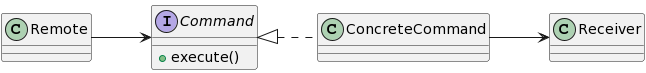
\includegraphics[scale=0.4]{img/command.png}\par}
\section{Design Principles}
\subsection{Single responsibility principle}
A class should have only one reason to change. Should only have one responsibility and be able to describe what a class is doing in a single line.
\subsection{Open-close principle}
Objects should be open for extension, but closed for modification. When you split responsibiity of a class through the SRP, you should do it in a way that behaviour can be extended instead of having to modify it.
\subsection{Liskov's substitution principle}
Subtypes must be substitutable for their base types. You should use inheritance only when your superclass is substitutable by your subclass in all instances.
\subsection{Interface segregation}
The dependency of one class to another class should depend on the smallest possible interface. Only expose necessary elements of an interface to a class. Clients shouldn't be forced to implement interfaces they don't use. Since a class can implement multiple interfaces, have small interfaces based on groups of methods, each serving one submodule, instead of one large interface. You can also have interfaces extend another interface to build specific interfaces. Allows you to split the responsibility of a class for SRP without violating LSP. 
\subsection{Dependency inversion (design for interfaces)}
Depend on abstractions (interfaces) instead on concrete classes. Higher level modules should depend on interfaces of lower level modules, not directly on the lower level modules.
\section{MIS Template}
\subsection{Uses}
\begin{itemize}
\item Imported constants, data types, and access programs.
\end{itemize}
\subsection{Syntax}
\begin{itemize}
\item Exported constants\\
\item Exported types\\
\item Exported access routine (routine name, input and output parameter types, and exceptions in a table)
\end{itemize}
\subsection{Semantics}
\begin{itemize}
\item State variables (global variables)\\
\item State invariants (predicates using state variables where after every access routine call, should remain true)\\
\item Assumptions\\
\item Access routine semantics (transition = changing state variables (e.g. transition: this.start, this.end := start, end), output = output of the access routine (e.g. output: out := this), exception = exception (e.g. exception: none))\\
\item Local functions, types, constants (declared for specification purposes only, not available at runtime)\\
\item Considerations (other information like "consider doing x to y to do z")\\
\end{itemize}
\section{Testing}
{\centering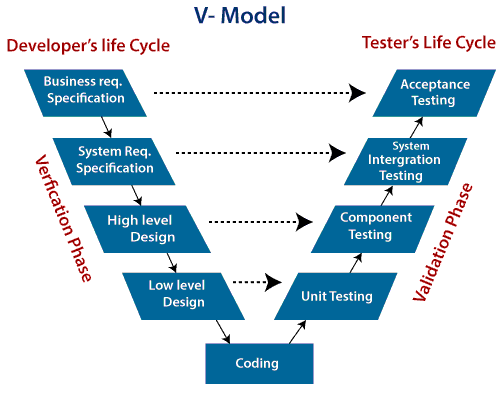
\includegraphics[scale=0.3]{img/V-model.png}\par}
\textbf{Unit testing}: testing individual methods/functions with inputs and expected outputs. Every successful test gives confidence in the code's correctness, but it never guarantees correctness. Should use Hoare triples, but you can't for black box testing.\\
\textbf{Black box testing}: you have a method with a general idea of what it does, but you don't know how it works and you can only give it inputs and look at the output. You can start writing black box tests without the code being done.\\
\textbf{White box testing}: you have a method and its code.\\
\textbf{Statement coverage}: your test cases cause each statement (of the method's code) to be executed at least once.\\
\textbf{Edge coverage}: same as statement coverage, but refers to a code graph (covers each edge of the code graph at least once).\\
\textbf{Code graph}: convey the program as a graph with branches from conditional statements (edges = statements).\\
\textit{A test suite has statement coverage iff it has edge coverage.}\\
Statement and edge coverage still aren't enough since it may miss errors in the code.\\
\textbf{Path coverage}: a test suit has path coverage if it traverses all pahts from the start node to the end node(s) at least once in the code graph. Often times path coverage is too large (e.g. a circuit with 20 boolean inputs).\\
\textbf{Static testing}: reading the code.\\
\textbf{Dynamic testing}: running the code.
\subsection{Number of bugs (fault seeding)}
If $N$ is the actual number of bugs, you found $C$ bugs, another team found $M$ bugs and you both found $S$ common bugs, then the actual number of bugs ranges from $N_1=(C-S)M/S$ to $N_2=(M-S)C/S$.\\
Assumes that $M/S = N/(C-S)$. I.e. the ratio of marked fish to caught marked fish resembles actual fish to caught actual fish, but it might not be really true since marked fish are easier to catch.
\end{multicols}
\end{document}